\documentclass[10pt]{report}
\usepackage[utf8]{inputenc}
\usepackage[top=2cm, bottom=2cm, left=2cm, right=2cm]{geometry}
\usepackage[francais]{babel}
\usepackage{helvet}
\usepackage[T1]{fontenc}
\usepackage{graphicx}
\usepackage{subcaption}
\usepackage{lmodern}
\usepackage{listings}
\usepackage{wrapfig}
\usepackage[colorlinks=true, linkcolor=black, urlcolor=blue, breaklinks, pagebackref, citebordercolor={0 0 0}, filebordercolor={0 0 0}, linkbordercolor={0 0 0}, pagebordercolor={0 0 0}, runbordercolor={0 0 0}, urlbordercolor={0 0 0}, pdfborder={0 0 0}]{hyperref}  %désactive les cadres autour des liens
\usepackage{etoolbox}
\renewcommand{\familydefault}{\sfdefault}

% Supprime l'espace avant l'en-tête des chapitres
\makeatletter
% les chapitres normaux
\patchcmd{\@makechapterhead}{\vspace*{50\p@}}{}{}{}	
% les chapitres étoilés
\patchcmd{\@makeschapterhead}{\vspace*{50\p@}}{}{}{}
\makeatother


\begin{document}

\begin{titlepage}	
	\flushleft
	\begin{figure}[!h]
		
\includegraphics[height=1.8cm]{Reports/figures/logo_insa_cvl.png}
		\hfill
		
\includegraphics[height=3cm]{Reports/figures/logo_biomedia.png}
	\end{figure}
	\centering
	\vspace{2cm}
	{\scshape\Large Stage industriel de 4ème année\par}
	\vspace{1.5cm}
	{\huge\bfseries Développement d'une bibliothèque mathématique performante pour le traitement d'images médicales\par}
	\vspace{2cm}
	{\Large\itshape Élève ingénieur: François PIAT\par}
		\vspace{1cm}
	\begin{figure}[!h]
		\begin{center}
			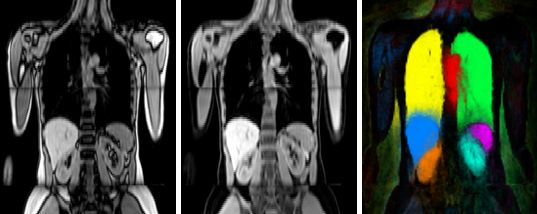
\includegraphics[width=13cm]{Reports/figures/biomedia_image.png}
		\end{center}
	\end{figure}
	\vfill
	\flushleft
	Tuteur INSA: \hfill Tuteur BioMedIA: \par
	Julien \textsc{Olivier} \hfill Ghislain-Anthony \textsc{Vaillant}
	\vfill
	% Bottom of the page
	\centering
	{\large Année universitaire 2015 - 2016 \par}
\end{titlepage}

\section*{Remerciements}\newpage
\paragraph*{Résumé} % dans cet ordre
\paragraph*{Mots-clés}
\paragraph*{Abstract}
\paragraph*{Key-words}

% sommaire
\renewcommand\contentsname{Sommaire}
\tableofcontents

\newpage

\chapter*{Introduction}
\addcontentsline{toc}{chapter}{Introduction}
\chapter{Environnement de travail} 
	Le stage s'inscrivant dans un cadre de recherche, cette section présente le laboratoire dans lequel il s'est déroulé. En fin de section seront présentées les raisons de la genèse du stage.
	\section{Le laboratoire}
	%Le laboratoire BioMedIA est implanté sur le campus principal de l'Imperial College London, dans le quartier du South Kensington. Il fait partie du groupe de recherche en traitement visuel d'informations (Visual Information Processing) au sein du département informatique de l'université.
	%Cette section.... le cadre de travail,le contexte, justifie la genèse du stage
	\subsection{Imperial College London - Department of computing}
	% Inclure les figures , ne pas oublier les titres, et ne pas faire : "comme on voit ici :"
	\paragraph{Imperial College London}~\par ~\par %souligner la section ou l'on est
	L’Imperial College London (officiellement The Imperial College of Science, Technology and Medicine) est une université britannique fondée en 1907 par la fusion du City and Guilds College, de la Royal School of Mines et du Royal College of Science (tous fondés entre 1845 et 1878).\\ ~\par
    L'université possède au total 9 campus, tous situés à Londres, et dont la plupart sont implantés dans des sites hospitaliers.  
    Elle possède 5 départements administratifs et 4 branches techniques: ingénierie, sciences naturelles, business, et médecine.	Le campus principal est basé dans le quartier du South Kensington, et regroupe la branche d'ingénierie, de sciences naturelles, d'arts et de business. C'est sur ce campus que le département d'informatique est donc basé. 
	\begin{figure}[h!]
		\begin{center}
			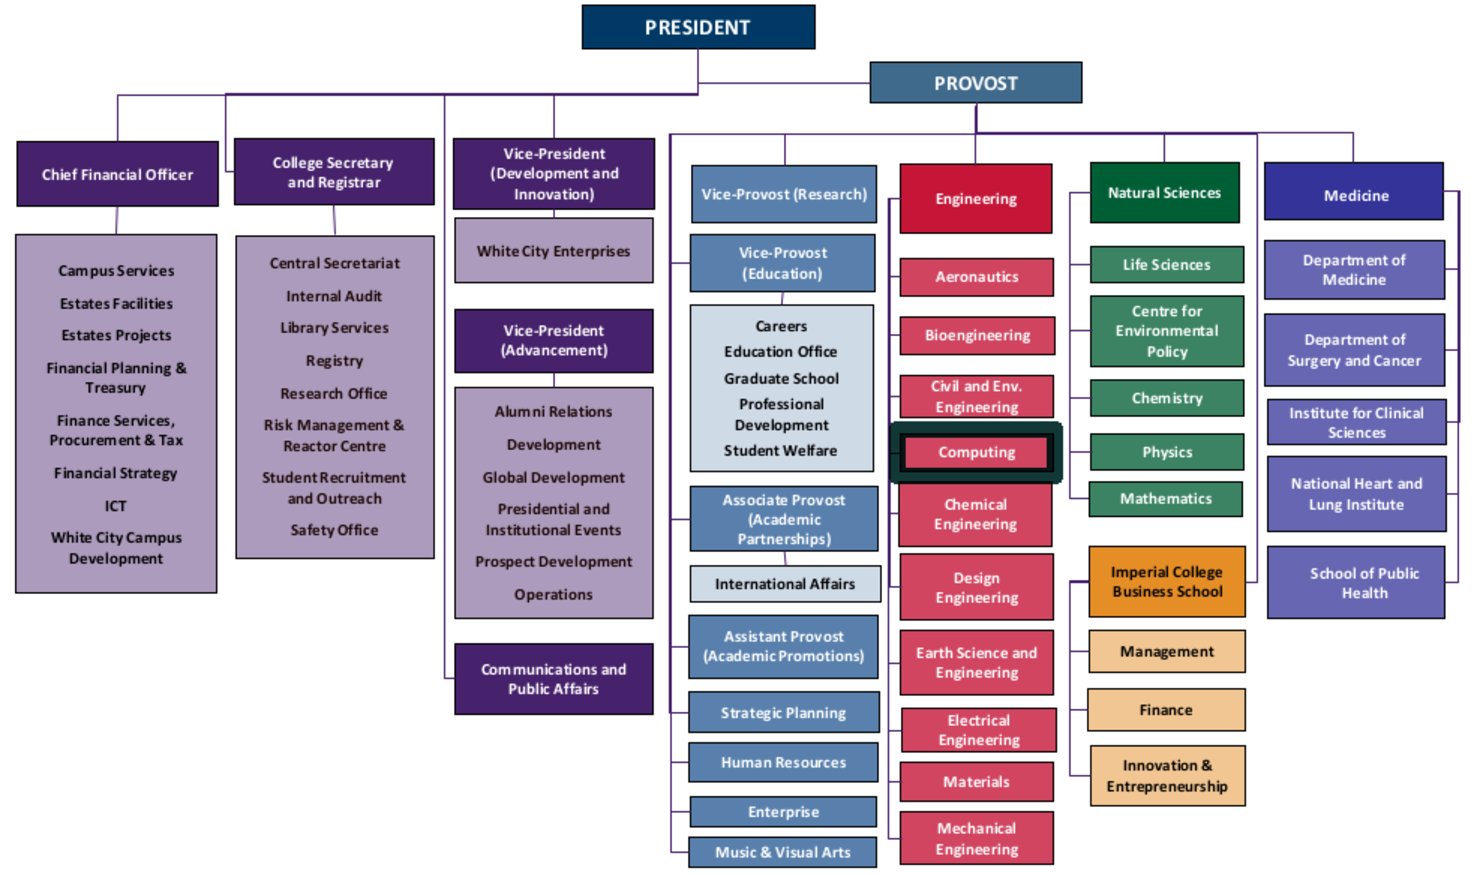
\includegraphics[width=18cm]{Reports/figures/College-Organisation.pdf}
		\end{center}
		\caption{Organigramme de l'Imperial College London \\ \textit{Le département de computing, encadré en noir, se situe dans la branche d'ingénierie (en rouge) de l'université.}}
		\label{Organigramme de l'Imperial College London}
	\end{figure}
	


%classifier les idées
	
	\paragraph{Department of computing}~\par~\par
	Le département d'informatique est divisé en 5 groupes de recherche : %decrire les branches
	\\{$\bullet$}\textit{\textbf{Logic and Artificial Intelligence:}} la recherche en Logic and Artificial Intelligence englobe des études fondamentales de logique et une variété de disciplines en intelligence artificielle.
	\\{$\bullet$}\textit{\textbf{Distributed Software Engineering:}}	la recherche dans le domaine du Distributed Software Engineering aborde la conception de systèmes distribués, adaptatifs et fiables.
	\\{$\bullet$}\textit{\textbf{Quantitative Analysis and Decision Science:}} la recherche en Quantitative Analysis and Decision Science varie de l'optimisation à l'ingénierie de performances, en passant par la des expériences de vérifications quantitatives ou de sécurité.
	\\{$\bullet$}\textit{\textbf{Programming Languages and Systems:}} Programming Languages and Systems est une section qui combine des travaux théoriques et pratiques en langages et architecture pour obtenir des logiciels rapides, et efficaces.
	\\{$\bullet$}\textit{\textbf{Visual Information Processing:}} la recherche en Visual Information Processing couvre une multitude de domaines, incluant la vision numérique, les graphiques, l'apprentissage automatique, et le traitement d'images médicales. 
	\begin{wrapfigure}[13]{r}{10cm}
		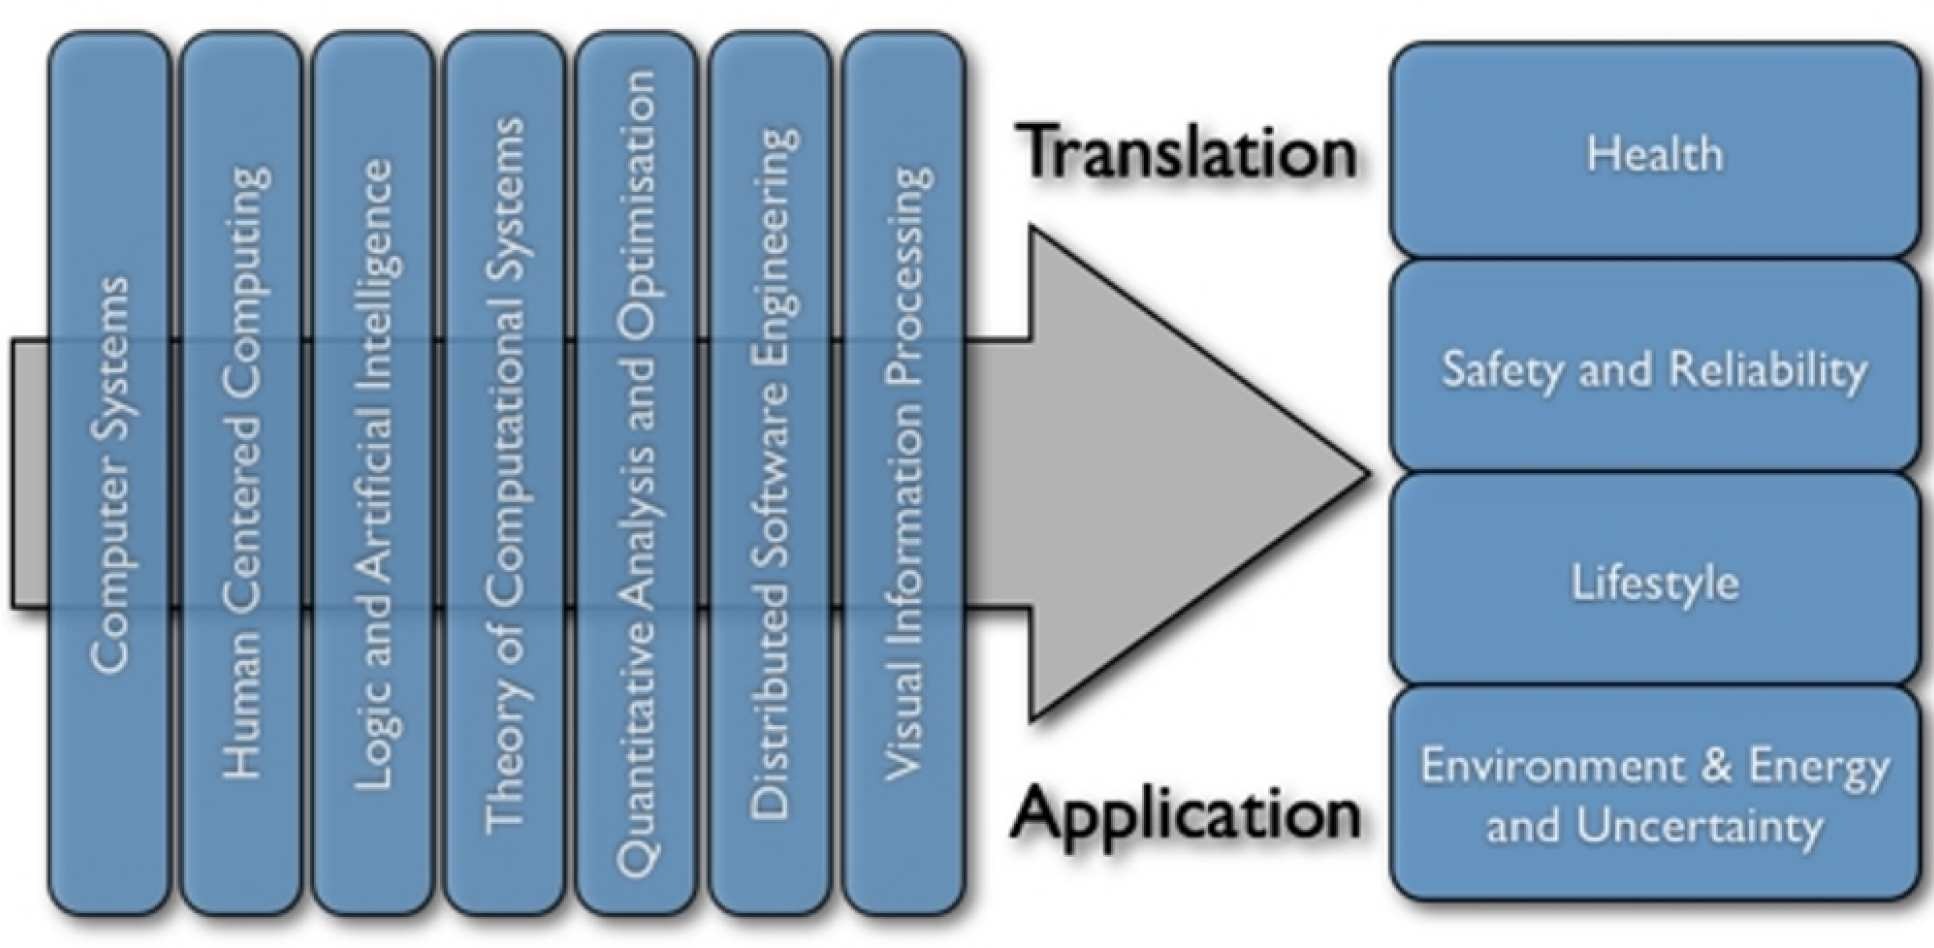
\includegraphics[width=9cm]{Reports/figures/research_strategy.jpg}
		\caption{Stratégie du département de recherche}
		\label{Stratégie du département de recherche}
	\end{wrapfigure}~\par~\par
	
	Les différentes spécialités citées précédemment sont articulées au sein du centre de recherche afin d'appliquer les résultats à d'autres domaines de recherche. Ces principales applications concernent les domaines de la santé, de la fiabilité/sécurité, de l'environnement, des modes de vie, de l'énergie et des incertitudes.
	\\
	\\
	\subsection{BioMedIA}
%	Synopsis, détail des activités du laboratoire
	
	La mission du groupe BioMedIA est de développer de nouvelles techniques de
	calcul pour l'analyse d'images biomédicales. Le groupe se concentre sur des
	domaines de recherche de pointe, y compris:\\

	{$\bullet$} Le développement d'algorithmes d'acquisition, d'analyse et d'interprétation des images. En particulier dans les domaines du recalage, de la reconstruction,
	du suivi de mouvement, de la segmentation et de la modélisation. \\

	{$\bullet$} L'apprentissage machine pour l'extraction d'information clinique à partir
	d'images médicales. Les applications incluent le diagnostic assisté par
	ordinateur, la planification automatisée de traitement médical, ou encore la thérapie et les interventions guidées par ordinateur. \\

	Le laboratoire s'intéresse particulièrement à l'imagerie et les technologies de
	traitement informatique qui permet de mieux comprendre le
	développement du cerveau humain, l’évolution des maladies mentales et le
	diagnostic des patients atteints de maladie cardiovasculaire.
	
	
	\section{Cadre du projet} % présentation de MIRTK, de ses applications, de son architecture(modules, fonctions...).
	\subsection{Medical Image Registration Toolkit (MIRTK)}~\par~\par
	Le Medical Image Registration Tool-Kit (abrégé MIRTK) est un logiciel open-source de traitement d'images médicales codé en C++ et utilisé par des chercheurs dans le milieu médical. Ces chercheurs sont, grâce à ce logiciel, aptes à analyser et manipuler des images en 2,3 ou 4 dimensions.   \\ 
	
%	Afin de rester pertinent pour ces chercheurs, MIRTK nécessite donc une maintenance et une amélioration continue.
%	
	L'utilisation de MIRTK est basée sur l'appel de lignes de commandes, incluant le nom de la fonction, les paramètres et les arguments nécessaires, et propres à chacune des fonctions. Par exemple, la ligne de commande suivante va rogner une image :
	\begin{lstlisting}
mirtk extract-image-region input.nii.gz output.nii.gz -Rx1 50 -Rx2 40 -Ry1 250 -Ry2 250
	\end{lstlisting}
	Sur cette ligne de commande:
	\\{$\bullet$} "mirtk" indique que l'on souhaite utiliser une fonction de MIRTK
	\\{$\bullet$} "extract-image-region" appelle la fonction de rognage
	\\{$\bullet$} "input.nii.gz" indique l'emplacement de l'image d'entrée, idem pour la sortie avec "output.nii.gz". Ces fichiers sont au format NIFTI (ici, ces images sont aussi compressées), seul format pris en charge par MIRTK.
	\\{$\bullet$} "-Rx1 50" signifie "retirer 50 pixels sur l'axe x, pour la première direction" (idem pour "-Rx2 40 -Ry1 250 -Ry2 250"). 
	L'action de cette ligne de commande est visualisable sur la Figure \ref{Effet de la fonction "extract-image-region"}.
	\begin{figure}[h!]
		\centering
		\begin{subfigure}{.5\textwidth}
			\centering
			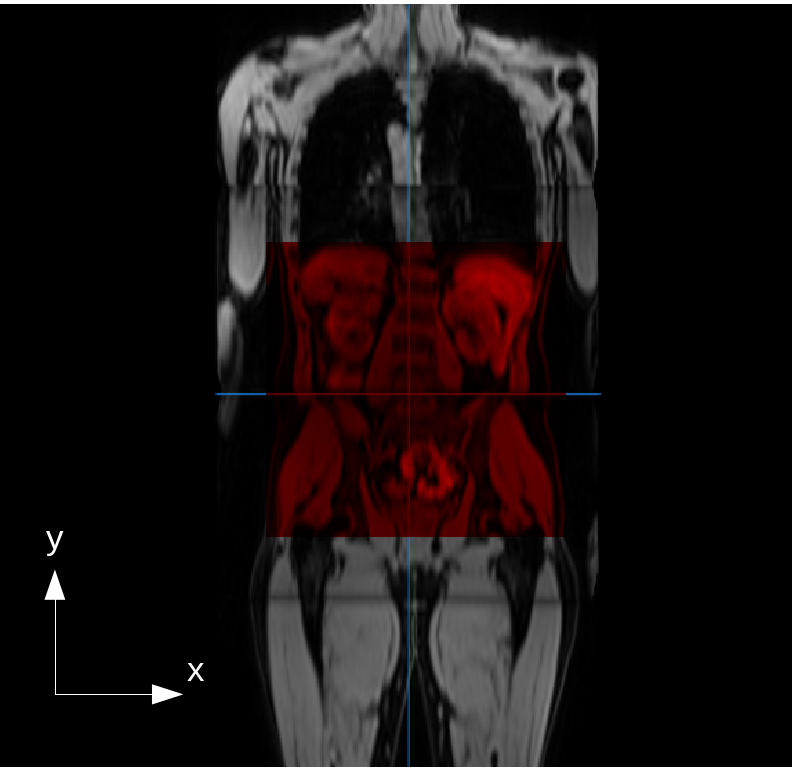
\includegraphics[width=5cm]{Reports/figures/mirtkextractregion1d.png}
			\caption{Image d'entrée}
			\label{Image d'entrée}
		\end{subfigure}%
		\begin{subfigure}{.5\textwidth}
			\centering
			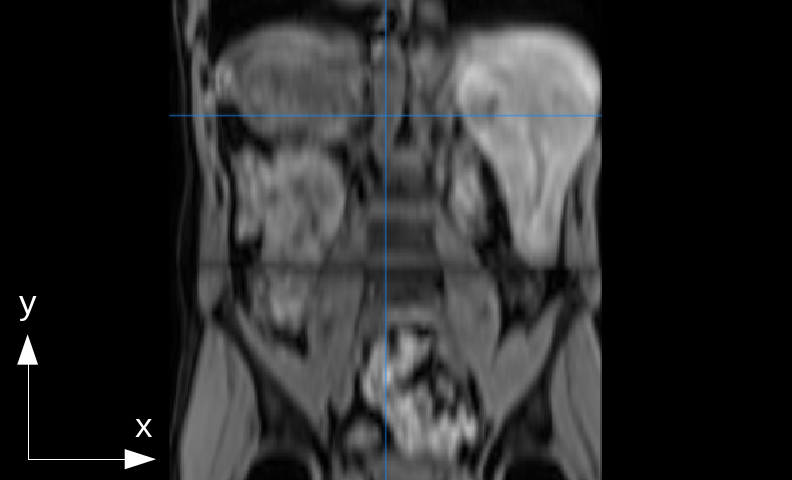
\includegraphics[width=7cm]{Reports/figures/mirtkextractregion2_1d.png}
			\caption{Image de sortie}
			\label{Image de sortie}
		\end{subfigure}
		\caption{Effet de la fonction "extract-image-region"}
		\label{Effet de la fonction "extract-image-region"}
	\end{figure}~\par
	Chaque fonction de MIRTK est exécutée par un fichier binaire qui a été généré par le fichier d'application associé. Tous ces fichiers sont d'ailleurs répertoriés dans un dossier \textit{Applications} et font appel à certaines dépendances, qui sont réparties en 7 modules : \textit{Common, Image, I/O, Numerics, PointSet, Registration} et \textit{Transformation}. Ces différents modules représentent le lien entre le back-end de MIRTK et son corps. Le recalage d'image (Registration) est l'une de ses principales fonctions. %Cependant, n'étant pas seul sur le marché du logiciel de traitement d'images, MIRTK nécessite une maintenance et une amélioration continue pour rester pertinent.\\
	
%	\begin{figure}[h!]
%		\begin{center}
%			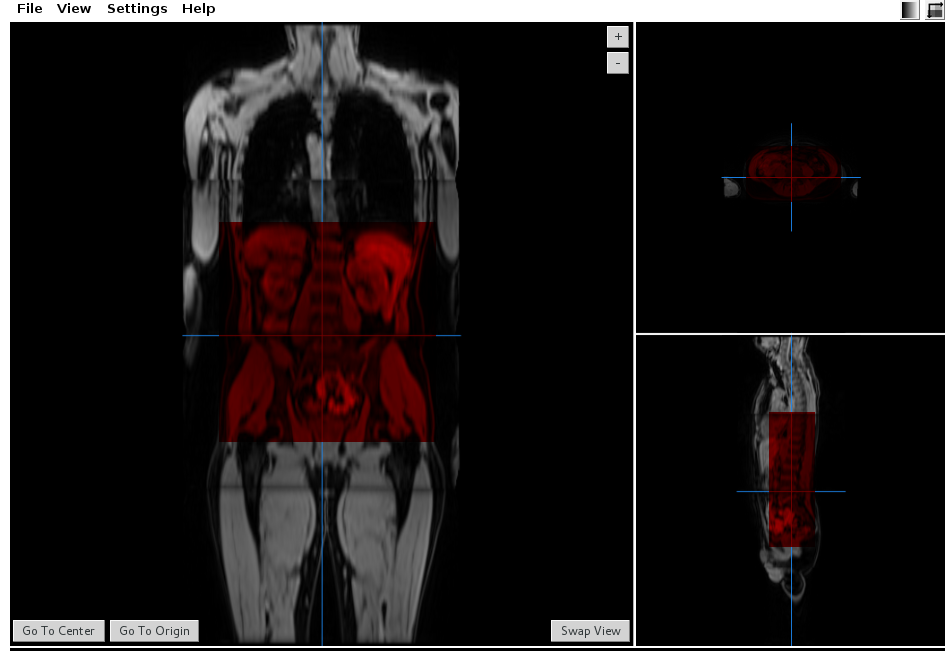
\includegraphics[width=10cm]{Reports/figures/mirtkextractregion1.png}
%		\end{center}	
%		\caption{Image fournie en entrée de "extract-image-region"}
%		\label{Image fournie en entrée de "extract-image-region"}
%	\end{figure}~\par
	
%	Comme on peut le constater ci-dessus, l'image en entrée du logiciel est une image en 3 dimensions. C'est d'ailleurs ce qui fait la force de MIRTK: il peut agir sur des images en 2, 3, ou 4 dimensions (la quatrième dimension représentant le temps). L'image est ici en noir et blanc, mais des travaux de segmentations notamment, peuvent aussi bien utiliser des palettes de couleurs. Le cadre rouge est purement fictif et indique simplement les limites du rognage effectué.
	
%	\begin{figure}[h!]
%		\begin{center}
%			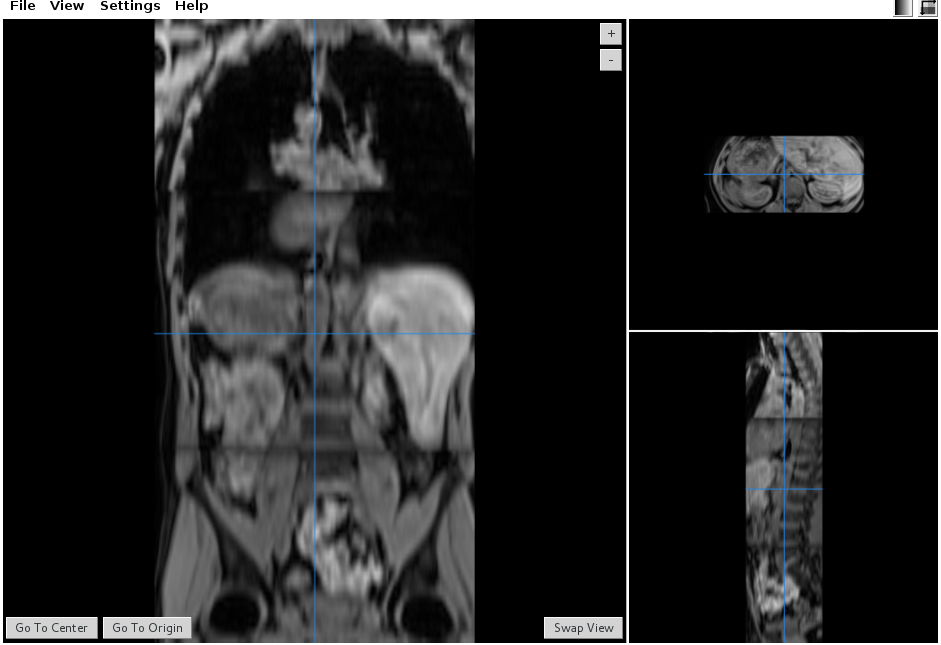
\includegraphics[width=10cm]{Reports/figures/mirtkextractregion2.png}
%		\end{center}	
%		\caption{Image obtenue après rognage 3D}
%		\label{Image obtenue après rognage 3D}
%	\end{figure}~\par 
	% mettre 

%	On notera que cet exemple est très loin de refléter l'ensemble des capacités du logiciel. En effet, MIRTK agit aussi bien sur des filtres d'images, que de transformations, de recalages, de conversions... % ne pas mettre ces points, reste exhaustif
	 % - logiciel de traitement d'image médicales, utilisé par les chercheurs en milieu médical.
	 % - stable mais nécessite une maintenance et une amélioration continue pour rester pertinent.
	 % - Intervention sur le module "Numerics", bibliothèque mathématique.
	 \subsection{UK BioBank}~\par
	 "UK BioBank" est le nom donné à un projet initié par plusieurs entités de recherche du Royaume-Uni . En collaboration avec le gouvernement britannique, ce projet prévoit de regrouper la plus grosse banque de données médicales du Royaume-Uni. En plus de données numériques, cette base de données regroupera aussi des dizaines de données extra-médicales pour chaque patient. Ceci pourrait permettre, après analyse, de pouvoir corréler des comportements individuels communs à une ou plusieurs maladies graves. ~\par~\par
	 
	 MIRTK à le potentiel pour s'inscrire dans ce projet, à long terme, en tant que "boite à outils" officielle, permettant d'analyser et d'étudier les grandes quantités de données visualisables de UK BioBank. ~\par~\par
	 %paragraphe : "d'ou vient le stage: lier MIRTK à BioBank"
	 Le projet de UK BioBank compte obtenir des données relatives à 100 000 individus. Parmi ces données seront inclues des images médicales qu'il faudra analyser. A l'heure actuelle, MIRTK est adapté pour manipuler quelques dizaines de ce type d'images, mais à besoin d'une amélioration de ses performances. Dans ce cadre, le but principal de ce stage est donc de commencer la démarche d'amélioration du logiciel en terme de design et de performances.
\chapter{Objectifs et cahiers des charges}
	\section{Problématique} %Inclure contexte du projet, avec la raison pour laquelle ce projet est nécessaire.
%	%(back-end math) dépendances externes : eigen et boost + noyaux internes implémentés via TBB => inconsistence => parrallélisation existante floue , efficacité = ? performances=? => profilage	===> n'utiliser qu'une seule dépendance (externe) : ArrayFire qui peut amener l'optimisation via GPU (résumer ça en 3 points majeurs) 
%	
	Dans l'optique de préparer MIRTK à son insertion dans le projet UK BioBank, et d'obtenir des résultats concluant relativement rapidement, on pourra distribuer les calculs à différentes échelles : \\
	\t - sur un slurm, qui correspond a un réseau local de machines.\\
	\t - sur un High Performance Computing (HPC), qui s'étant à tous le réseau de machines de l'Imperial college, mais qui est un service payant.\\
	\t - sur un cloud, soit un serveur que l'on loue à une entreprise qui propose un tel service, telles que Google ou Amazon.\\ ~\par
	Ces différents supports de calculs pourront accélérer l'obtention des résultats, sachant que la liste précédente est classée de manière croissante concernant la rapidité d'exécution. Cependant, le HPC ou un cloud serait payant, avec un prix croissant selon le temps d'exécution. Semblablement, un slurm utilise les performances d'autres machines, qui, elles-même peuvent éventuellement être déjà occupées par l'exécution d'un autre logiciel. C'est pourquoi une exécution de MIRTK devra être la plus rapide possible, puisque, dans tous les cas, elle sera répétée un grand nombre de fois sur le support choisi.
	
	%pb : 100 000 executions : ca fait trop pour MIRTKtemps d'execution : les executions sont sous traitées, donc ils doivent etre cours pour eviter de payer trop : slurm (groupe de machine en local) => HPC (echelle de l'université, payant) => cloud (google amazon, payant), 
	\vspace{-0.5cm}
	\begin{wrapfigure}[20]{r}{9cm}
		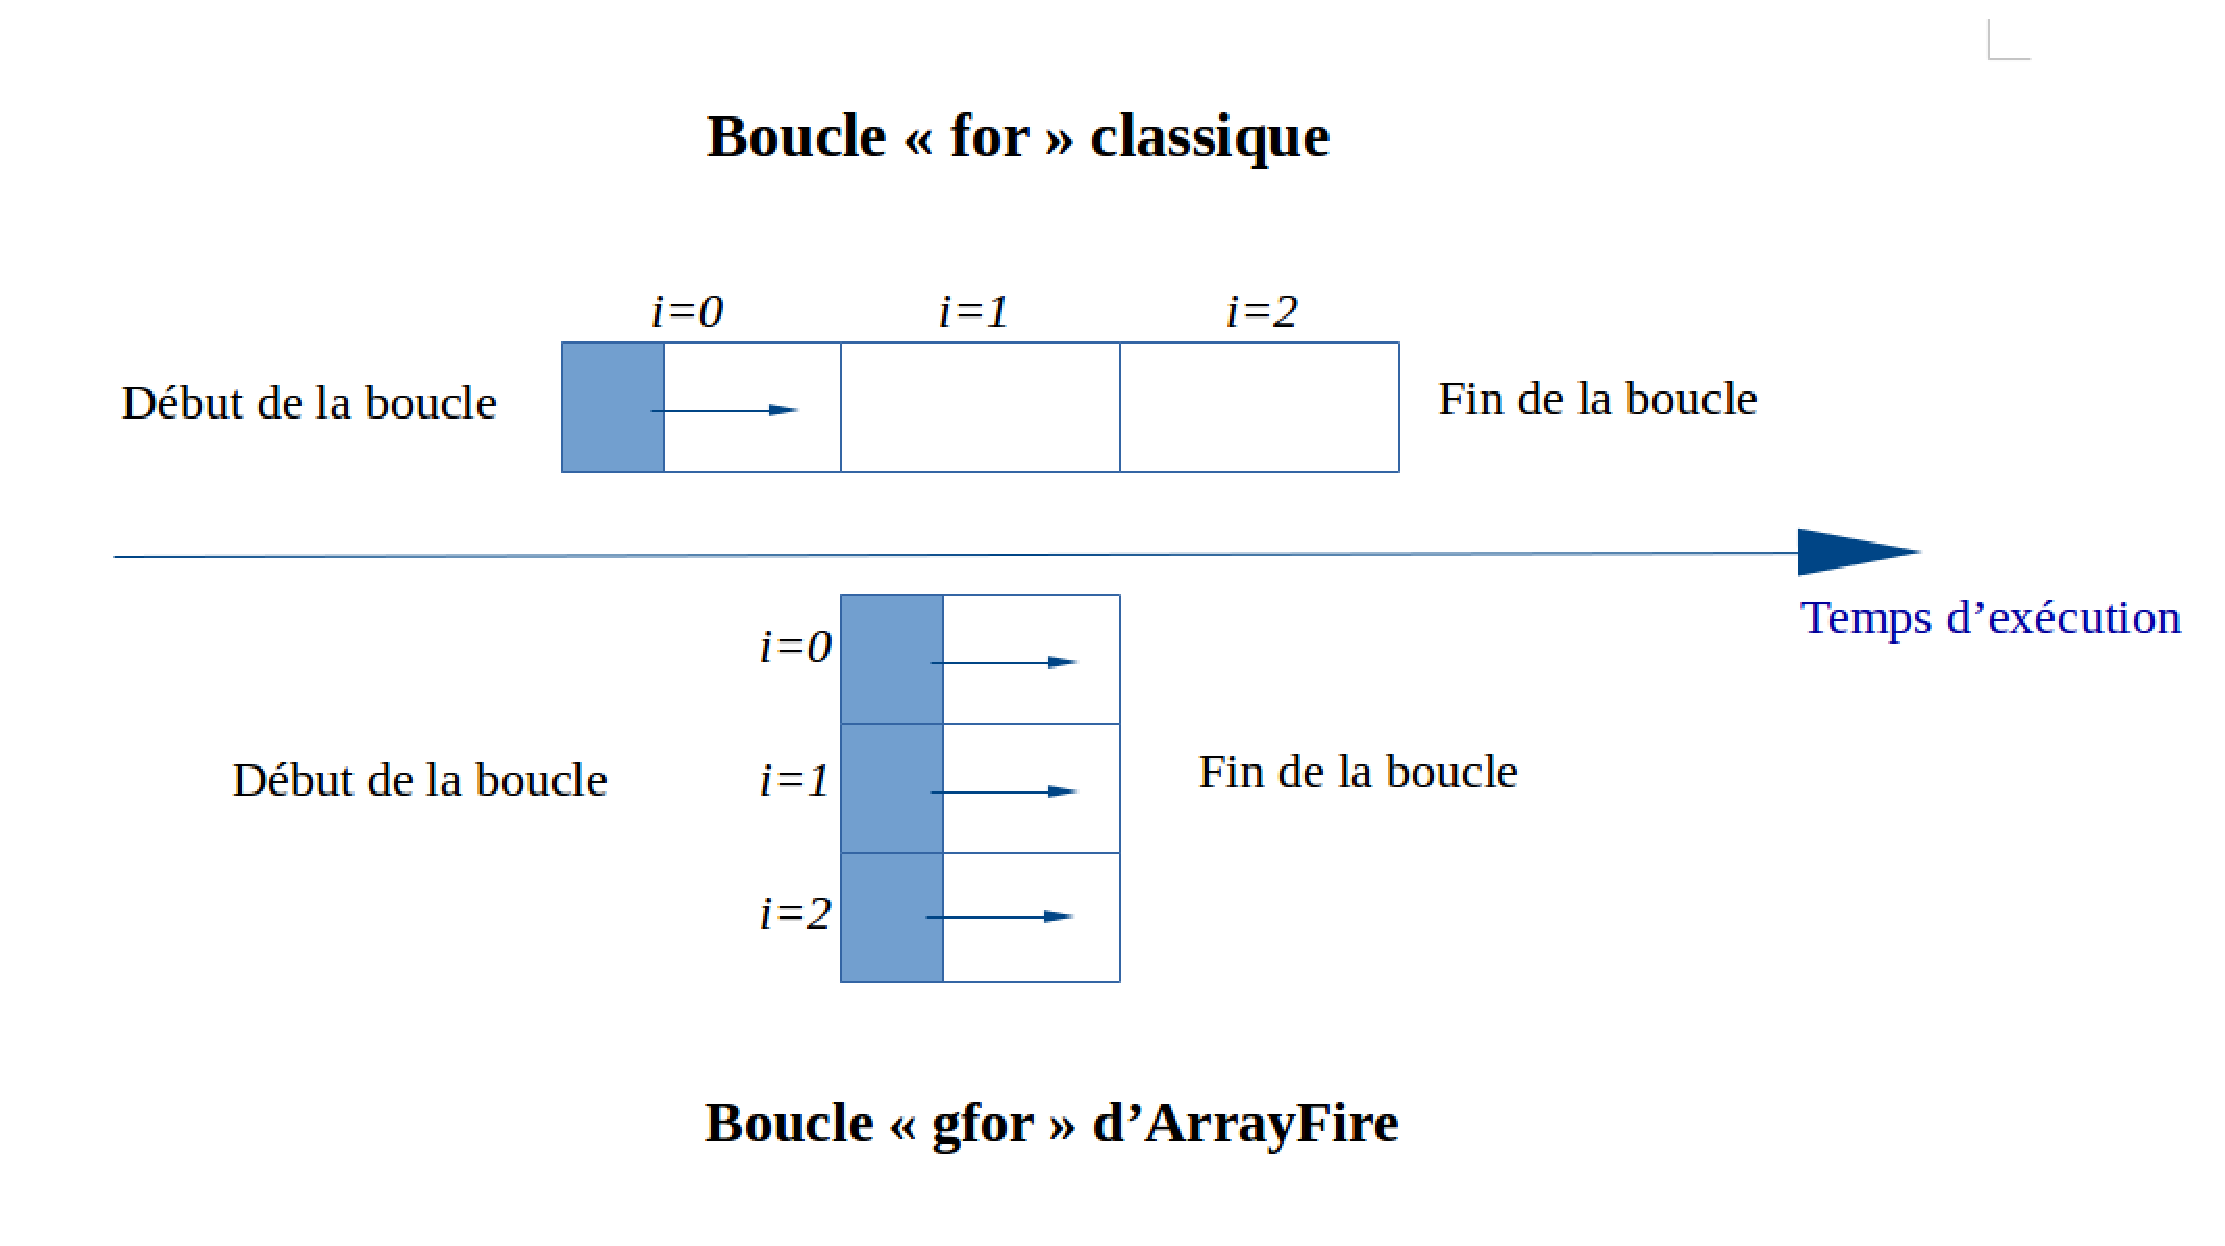
\includegraphics[width=10cm]{Reports/figures/gfor.eps}	
		\caption{Fonctionnement d'une boucle en parallèle}
		\label{Fonctionnement d'une boucle en parallèle}
	\end{wrapfigure}
	~\par~\par
	Par conséquent, le secteur sur lequel il faudra se pencher sera donc la réduction du temps d'exécution des fonctions du logiciel. Pour cela, MIRTK utilise une technique d'optimisation appelée "la parallélisation" d'un code. A l'inverse de l'exécution sérialisée, le principe de la parallélisation est d'assigner plusieurs threads dédiés à la commande appelée. Une fois assignés, chaque thread reçoit une quantité de "blocks" de code a exécuter. Chaque thread pourra donc traiter un block indépendamment du reste de l'exécution. Ainsi, plus la quantité de threads utilisée est grande, plus l'exécution sera accélérée. La figure \ref{Fonctionnement d'une boucle en parallèle} ci-contre représente ce principe avec des blocks de 2 itérations.\\

	La problématique du stage s'axera sur une optimisation de MIRTK au niveau des couches logicielles de bas niveau. Le logiciel, pour opérer chacune de ses fonctions, fait appel des dépendances mathématiques, implémentées dans le module \textit{Numerics}. La majeure partie du stage concernera donc ce module de MIRTK, c'est-à-dire les fonctions utilisant majoritairement des opérations matricielles.\\
	\section{Cahier des charges}
	La réduction du temps d'exécution est l'objectif principal du stage. Pour cela, il va falloir travailler sur 3 plans principaux : \\
	\\{$\bullet$} La compatibilité avec différents back-end, que ce soit pour processur (CPU) ou carte graphique (GPU). A l'heure actuelle, la gestion des back-end GPU n'est pas assurée par le logiciel. Le rendu idéal serait de laisser MIRTK gérer automatiquement cet aspect, en vérifiant la présence d'une carte graphique sur l'ordinateur (sinon utiliser le CPU), puis le laisser choisir entre CPU et GPU pour des performances optimales. Si, par exemple, un ordinateur possède une bonne carte graphique, MIRTK devra être apte à le détecter, et donc de l'utiliser.\\
	\\{$\bullet$} Garder l'intégrité et la transparence du code de MIRTK. Il sera imposé de garder les mêmes fonctions (ainsi que leurs arguments) et la même API. Pour conserver cela, il faudra garder une transparence entre le code de MIRTK et la gestion de différents back-end. C'est-à-dire que l'implémentation la plus haut niveau des fonctions du logiciel devra rester inchangée.\\
	\\{$\bullet$} Dans la mesure du possible, les fonctionnalités qui auront été dupliquées pendant le stage devront être supprimées, avec idéalement, la suppression d'une ou plusieurs dépendances du logiciel.
	
	
%	Lister les attentes et les contraintes du projet.

%gpu/cpu supportés
%Ne pas porter atteinte a la clarté du code
%Si possible, remplacer les dependances dupliquant les fonctionnalités introduites
%	ArrayFire pourrait être la bibliothèque la plus adaptée pour ce genre de situation puisqu'elle est similaire à l'actuelle bibliothèque EIGEN, mais en permettant l'optimisation du logiciel. Pour palier cette faiblesse d'EIGEN, TBB était nécessaire, mais pas avec ArrayFire. De plus, ArrayFire ajoute la possibilité de gérer le changement de back-end afin de travailler sur un GPU (carte graphique), ou sur un CPU (processeur).\\
%	\\
%	Avec cette bibliothèque, il va être possible de réaliser les points suivants:\\ 
%		\\{$\bullet$} Revoir les fonctions les plus coûteuses en ressources et dont les performances sont les plus médiocre, en les recodant avec ArrayFire.\\
%		\\{$\bullet$} Supprimer intégralement toute dépendance à TBB puisque la parallélisation du code se fera exclusivement avec ArrayFire.\\
%		\\{$\bullet$} La programmation sera réalisée de manière transparente, c'est-à-dire que MIRTK doit réaliser les mêmes fonctions et garder le même front-end même si le code plus en profondeur est modifié. En revanche, il sera possible d'ajouter des options d'exécution, notamment en ce qui concerne la gestion des back-end.\\
%		\\{$\bullet$} Plusieurs benchmarks devront affirmer la pertinence du nouveau code de MIRTK en comparant les test de performances avant et après l'intégration d'ArrayFire.\\
%%(Le délivrable sera composé IDEALEMENT de 2 backends, l'un AF et l'autre EIGEN. En fonction des applications, un switch automatique entre chaque structure sera appelé en dur grâce à des commandes pré-proc.) => étape bonus
%		\\{$\bullet$} A l'issue du stage, s'il reste suffisamment de temps pour s'y intéresser, il serait idéal d'implémenter une fonctionnalité de changement automatique de back-end en fonction des performances de EIGEN et ArrayFire sur une fonction en particulier. En se basant purement sur un critère de performances, on pourrait par exemple avoir une génération de matrice initiée par EIGEN puis une rotation de matrice exécutée par ArrayFire. Les commandes de changement automatique de back-end seront idéalement codées dans le pré-processeur du code de MIRTK. Il restera tout de même une possibilité d'empêcher cette bascule automatisée (qui sera au final définie par défaut) par commande manuelle.
%	\\
%	\\
%	\textit{Je tiens à préciser que les différents points du cahier des charges listé ci-dessus sont idéaux. Ne sachant pas à quoi s'attendre lors de l'étude de MIRTK, il se peut que ces différents points se voient modifiés, en fonction de la difficulté, du temps requis ou encore de la possibilité de leur réalisation.} 
	\section{Stratégie employée}
	\subsection{Objectifs} 
%	Détailler les objectifs a atteindre idéalement.
%	- Ajouter ArrayFire à MIRTK, en remplaçant les fonctions d'EIGEN les moins adaptées par les fonctions d'AF. \newline
%	- Faire un profiling des fonctions concernées par TBB, et interpréter les résultats afin d'élaborer une stratégie pour implanter la programmation // d'AF.\newline
%	- Supprimer les TBB inutiles ou peu efficaces, et remplacer les autres par l'équivalent d'AF (gfor).\newline
%	\noindent Dans un premier temps, il faudrait analyser le code de MIRTK sur deux plans:\\~\par 
%	\t - Les fonctions utilisées par Eigen et qui seraient davantage adaptées avec ArrayFire \\~\par
%	\t - Les outils de parallélisation et l'utilisation de la bibliothèque TBB \\\\
%	La première étape se fera simplement en comparant l'utilisation directe de Eigen, ainsi que les interdépendances des fichiers MIRTK avec ceux de la bibliothèque. Cependant, la deuxième demandera une analyse plus approfondie: en plus d'une analyse de code tel que précédemment avec EIGEN, il faudra réaliser un "test de performance" sur certaines fonctions. Ce test est appelé un profilage (ou \textit{profiling} en anglais) et peut analyser différents critères. Ainsi pourrons-nous cibler les fonctions les plus urgentes à modifier, qui sont mal rédigées ou qui demande relativement trop de ressources.
%	A la suite de ce profilage sera donc élaboré un "plan d'attaque" pour savoir par quelle partie du projet commencer.
%	\t - A terme, après avoir retiré au maximum les dépendances de MIRTK avec TBB, on pourra commencer des tests de benchmarking afin de vérifier l'amélioration des performances.
	\subsection{Diagramme de GANTT}
	 => gantt chart prévisionnel (à mettre en français)
	\begin{figure}[h!]
		\begin{center}
			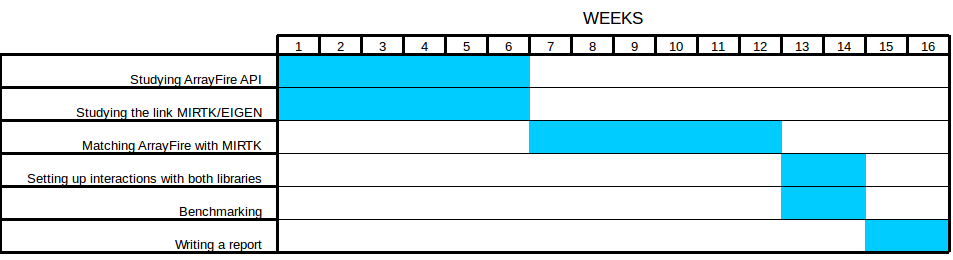
\includegraphics[width=18cm]{Reports/figures/estimated_gantt.png}
		\end{center}	
		\caption{Diagramme de GANTT prévisionnel}
		\label{Diagramme de GANTT prévisionnel}
	\end{figure}
\chapter{Réalisation}
%1. choix la dependance du module math => justification de Arrayfire.
%2. implémentation
%3. analyse de perf (profiling (démarche) + benchmark)
%	3.1 profiling
%	3.2 résultats
	\section{Choix et justification du module mathématique}

	
	\section{Implémentation}
	\subsection{Intégration du module mathématique}
	%	Programmation transparente entre Eigen et ArrayFire.
	%	Lister les fonctions principales à substituer.
	L'une des premières fonctions qui nous a attiré était un filtre, qui avait une implémentation assez simple (un simple produit de convolution de deux matrices). On a donc choisi de s'y intéresser avec ArrayFire.
	Ce filtre a été précédemment profilé, il s'agit de la fonction \textit{smooth-image}. La version de MIRTK était déjà implémentée de manière séparable, c'est-à-dire que le floutage est réalisé une dimension après l'autre, et c'est la méthode la plus optimisée pour un tel calcul. Cependant, on a tout de même remplacé l'implémentation existante en intégrant ArrayFire afin de comparer les performances et simplifier le code de la fonction. \\
	Dans un premier temps, une implémentation naïve a été initiée en reprenant à zéro le code de la fonction. Le floutage d'une image se fais par un produit de convolution entre la matrice représentant l'image, et le filtre (gaussien), qui est déclaré dans la fonction elle-même. L'implémentation naïve a donc été de réaliser ce produit de convolution de matrices en utilisant la fonction \textit{af::convolve}, qui réalise simplement la convolution du filtre 3D avec l'image 3D, comme on peut le voir ci-dessous:\\
	\begin{figure}[h!]
		\begin{center}
			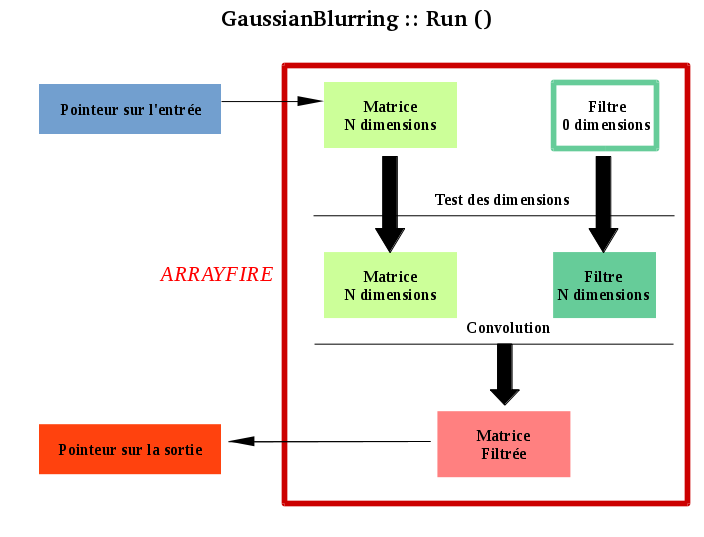
\includegraphics[width=11cm]{Reports/figures/gaussianblurring.png}
		\end{center}	
		\caption{Algorithme de flou gaussien incluant Arrayfire - Implémentation naïve}
		\label{Algorithme de flou gaussien incluant Arrayfire - Implémentation naïve}
	\end{figure}~\par
	Afin d'optimiser au maximum la fonction, il faut maintenant la ré-implémenter de la même manière que dans MIRTK, c'est-à-dire de manière séparable. Pour cela on effectue sur chaque dimension un produit de convolution sur la dimension 1 de la matrice, qu'on réordonne après, de telle manière à faire passer les valeurs de la dimension choisie en première dimension: \\
	\begin{figure}[h!]
		\begin{center}
			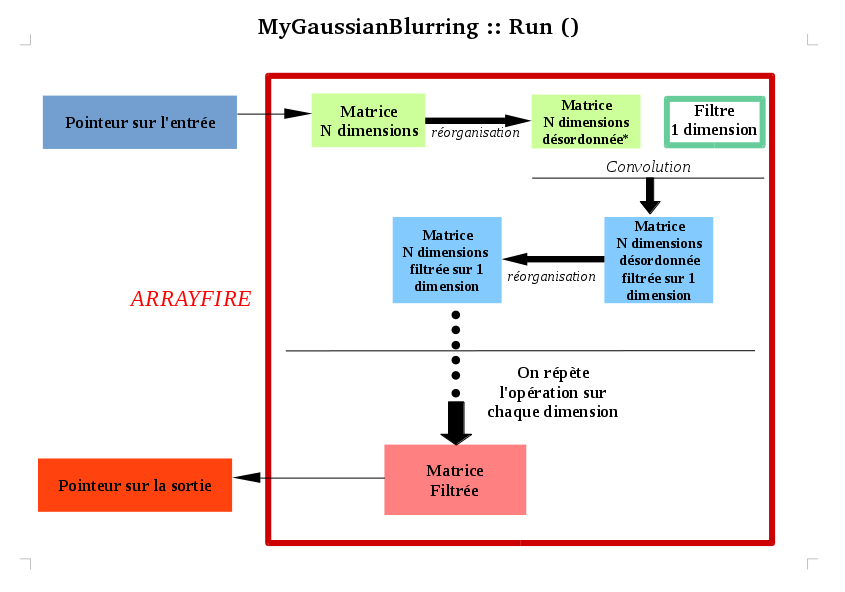
\includegraphics[width=12cm]{Reports/figures/mygaussianblurring.png}
		\end{center}	
		\caption{Algorithme de flou gaussien incluant Arrayfire - Implémentation optimisée}
		\label{Algorithme de flou gaussien incluant Arrayfire - Implémentation optimisée}
	\end{figure}~\par
	\subsection{Gestion de la programmation parallèle}
	%	Optimisation des threads et suppression de TBB au profit de ArrayFire.
	
	
	
	
	%	\newline
	%	Le contenus des sous-parties, ainsi que d'éventuelles d'autres sous-parties dépendront du résultat du profilage.
	
	\section{Analyse des performances}
		\subsection{Profilage}
	%	Définir le profilage et expliquer la nécessité d'une telle étape dans ce contexte\newline
		Lors du début de mon stage, il a fallu que je me familiarise avec les dépendances de MIRTK, mais aussi a son fonctionnement interne. C'est lors de cette étude préliminaire que mon tuteur et moi avons étudié, en plus de la bibliothèque EIGEN (destinée aux fonctionnalité mathématiques), la bibliothèque TBB, qui a pour but de mettre en place une parallélisation d'un logiciel. Constatant qu'ArrayFire était constitué de fonctions mathématiques déjà optimisées sur ce plan, il a été convenu de faire un profilage de MIRTK avant d'y intégrer ArrayFire afin de prioriser les points les plus coûteux en ressources de MIRTK. \\
	%	Les tests ont été effectués sur une machine dont les caractéristiques sont les suivantes : \newline
	%	{$\bullet$} \textit{Nombre de coeurs:} 8, 2 threads chacun\newline
	%	{$\bullet$} \textit{Cadence:} 1.6 GHz \newline
	%	{$\bullet$} \textit{Nombre de caches:} 4 \newline
	%	{$\bullet$} \textit{Taille des caches:}32k, 32k, 256K, 8192K \newline
		%ajouter le maximum de détails (RAM, nom du proc ...)\newline
		Pour une quantité réduite de tests, et afin de cibler les modèles d'utilisation de TBB à remplacer, on a pris l'une des fonctions les plus sollicitées dans MIRTK, il s'agit d'une fonction nommée \textit{transform-image}, et qui dispose de 5 options, définissant un type d'interpolation mathématique : Linéaire (par défaut), méthode voisin le plus proche (NN), gaussienne, sinus cardinal et B-Spline. \\
		On notera, de plus, que tous ces tests seront exécutés sur la même machine afin de garder des performances exactement semblables à chaque exécution.
		
		\subsection{Choix du profileur}~\par
		Afin de discerner au mieux les performances de MIRTK, le choix du profileur (l'outil faisant le profilage) était important. Le principal poste utilisée pour le profilage travaille sur un processeur INTEL, ce qui nous a convaincu de ne pas utiliser le profileur CodeXl puisque nous avons compris après installation qu'il ne fonctionnait qu'avec des processeurs AMD. On a ensuite basculé sur VTune, développé par les collaborateurs directs d'AMD, mais nous ne l'avons pas retenu non plus de part sa complexité d'installation sur l'ordinateur souhaité.
		
		Nous avons donc finalement choisi d'utiliser l'outil Callgrind de la suite VALGRIND (qui est open-source), capable d'analyser à la fois la quantité d'instructions envoyées au run-time, et aussi les fuites de cache.
		Ci-dessous est affichée l'interface utilisateur de Kcachegrind, qui est un outil permettant de visualiser de manière claire les résultats de Callgrind:
		\begin{figure}[h!]
			\begin{center}
				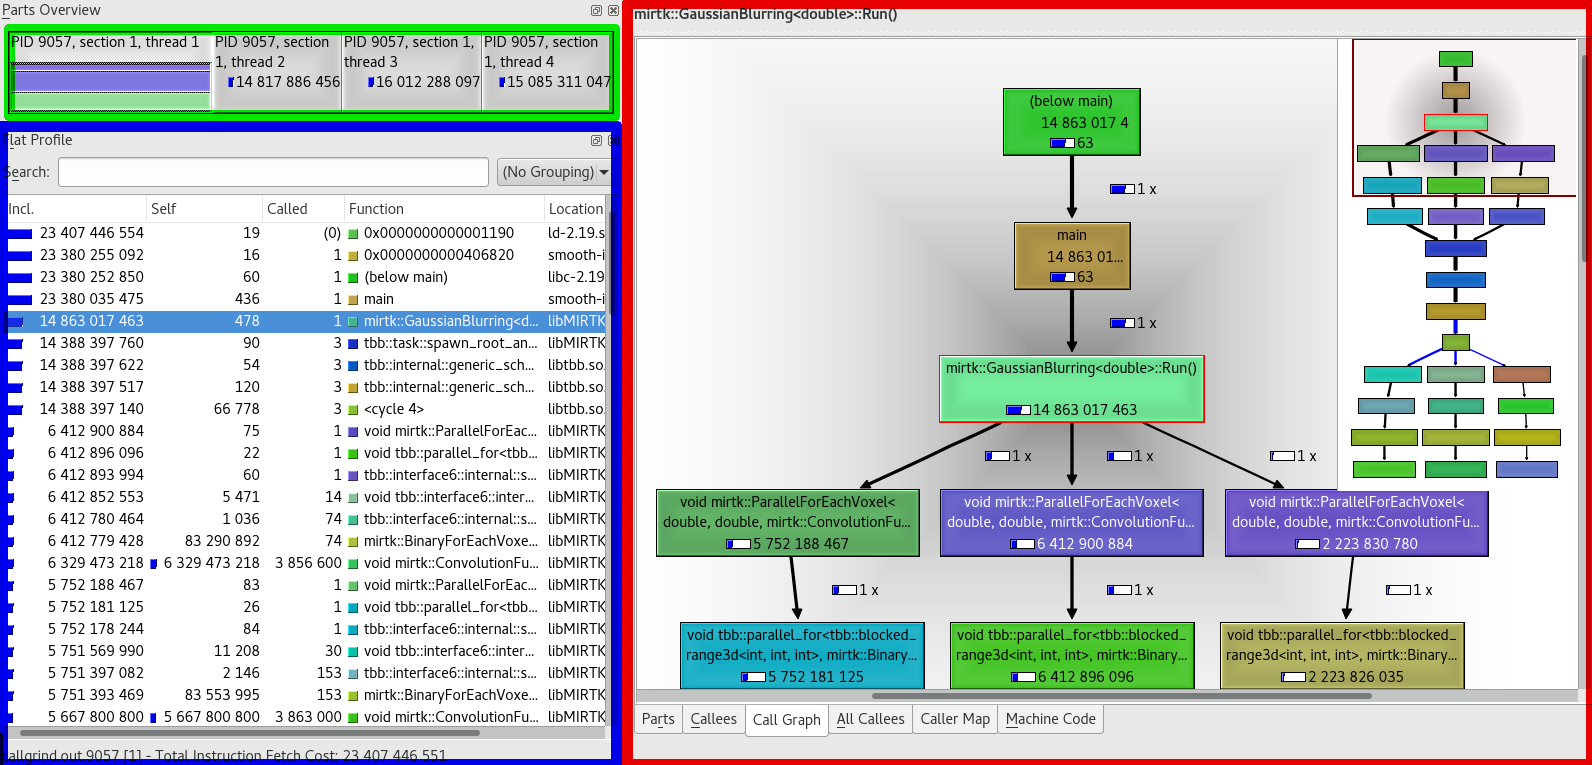
\includegraphics[width=13cm]{Reports/figures/UIkcachegrind.png}
			\end{center}	
			\caption{Interface de KCacheGrind pour le profilage}
			\label{Interface de KCacheGrind pour le profilage}
		\end{figure}~\par
		{$\bullet$} \textit{Cadre vert: } Dans cette partie est distinguée tous les threads qui ont exécuté une partie du code lié à l'exécutable étudié. Tous les threads ayant été utilisés dans ce cas, on peut constater que la machine fonctionne donc avec 4 coeurs. \newline
		{$\bullet$} \textit{Cadre bleu: } Ici est détaillé toutes les fonctions les plus coûteuses du thread sélectionné. \newline
		{$\bullet$} \textit{Cadre rouge: } Grâce à ce diagramme, on peut visualiser la pile d'appel des fonctions avant et après la fonction sélectionné dans le cadre bleu. Les onglets en bas de page sont d'autres représentations plus textuelles (et plus détaillées) de ce que montre le diagramme. \newline
		
		
	
	%	=> on identifie les fonctions sur lesquelles agir en premier
	%	On utilise Valgrind, qui, avec callgrind analyse la manière dont les caches sont utilisés.
	%	Expliquer le choix de valgrind, parmi les autres profileurs
	% => projet open-source multi-plateforme et disponible dans les packages linux, autres alternatives étudiées (VTUNE intel, installation compliquée, et codeXL, qui nécessite des proc AMD).\\
		
		
	
		
		\paragraph{Analyse du nombre d'instructions}
		
		\begin{wrapfigure}{r}{7.2cm}
			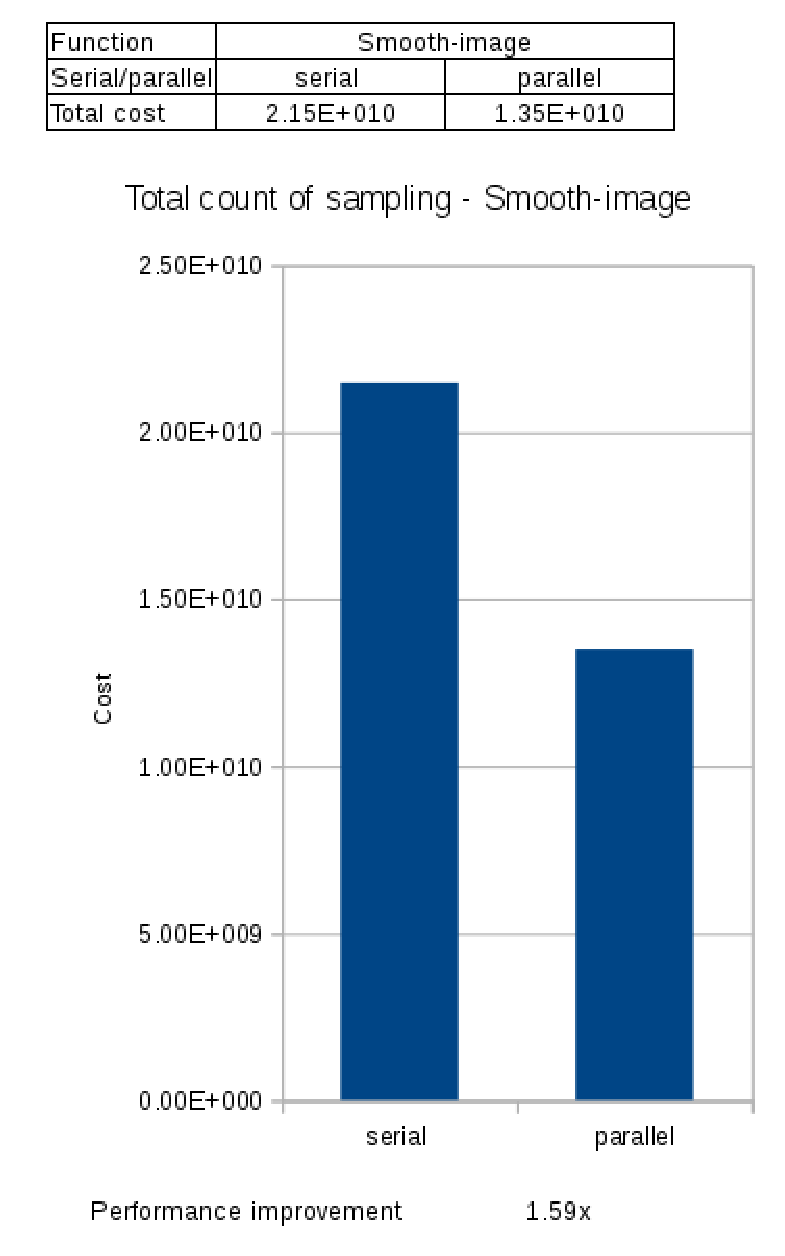
\includegraphics[height=9cm]{Reports/figures/smooth_image_costs.eps}
			\caption{Coût de la fonction de flou gaussien}
			\label{Coût de la fonction de flou gaussien}
		\end{wrapfigure}
		~\par~\par
		Dans un premier temps, on s'intéresse au critère le plus pertinent concernant les performances du logiciel. Le nombre d'instructions correspond à la quantité de commandes atomiques (au niveau binaire) exécutées par le CPU et pour chaque thread.
		Ainsi, on peut étudier l'efficacité de TBB en comparant le nombre d'instructions utilisées lorsque TBB est activé ou non. C'est ce qui est présenté sur l'image présentée ci-contre, en se focalisant sur une fonction de flou gaussien (nommée \textit{smooth-image}).\\
		Sur l'axe des ordonnées, on a le coût total en instruction de la fonction, appelée sur une machine précise, avec une entrée précise (ici une image 3D). Les résultats dépendent de ces deux critères.Cependant, le ratio entre les coûts de la fonction parallélisée et celle qui ne l'est pas reste sensiblement le même. Au bas de l'image, on peut voir qu'ici, la fonction à un taux d'amélioration de x1.59. L'ordinateur ayant exécuté cette fonction ayant 8 coeurs, on peut dire que ce résultat reflète une mauvaise parallélisation dans ce cas, car un logiciel bien optimisé aurait un taux d'amélioration proche de x8 (équivalent au nombre de coeurs utilisés).\\
		De même, ci-dessous, l'image décrit les performances de la fonction \textit{transform-image}. En revanche, ici, cette fonction possède une option qui permet de choisir son type d'interpolation mathématique. On a donc fait un test de coût d'instructions pour chaque interpolation et on a relevé ici le taux de performance associé:
		\begin{figure}[h!]
			\begin{center}
				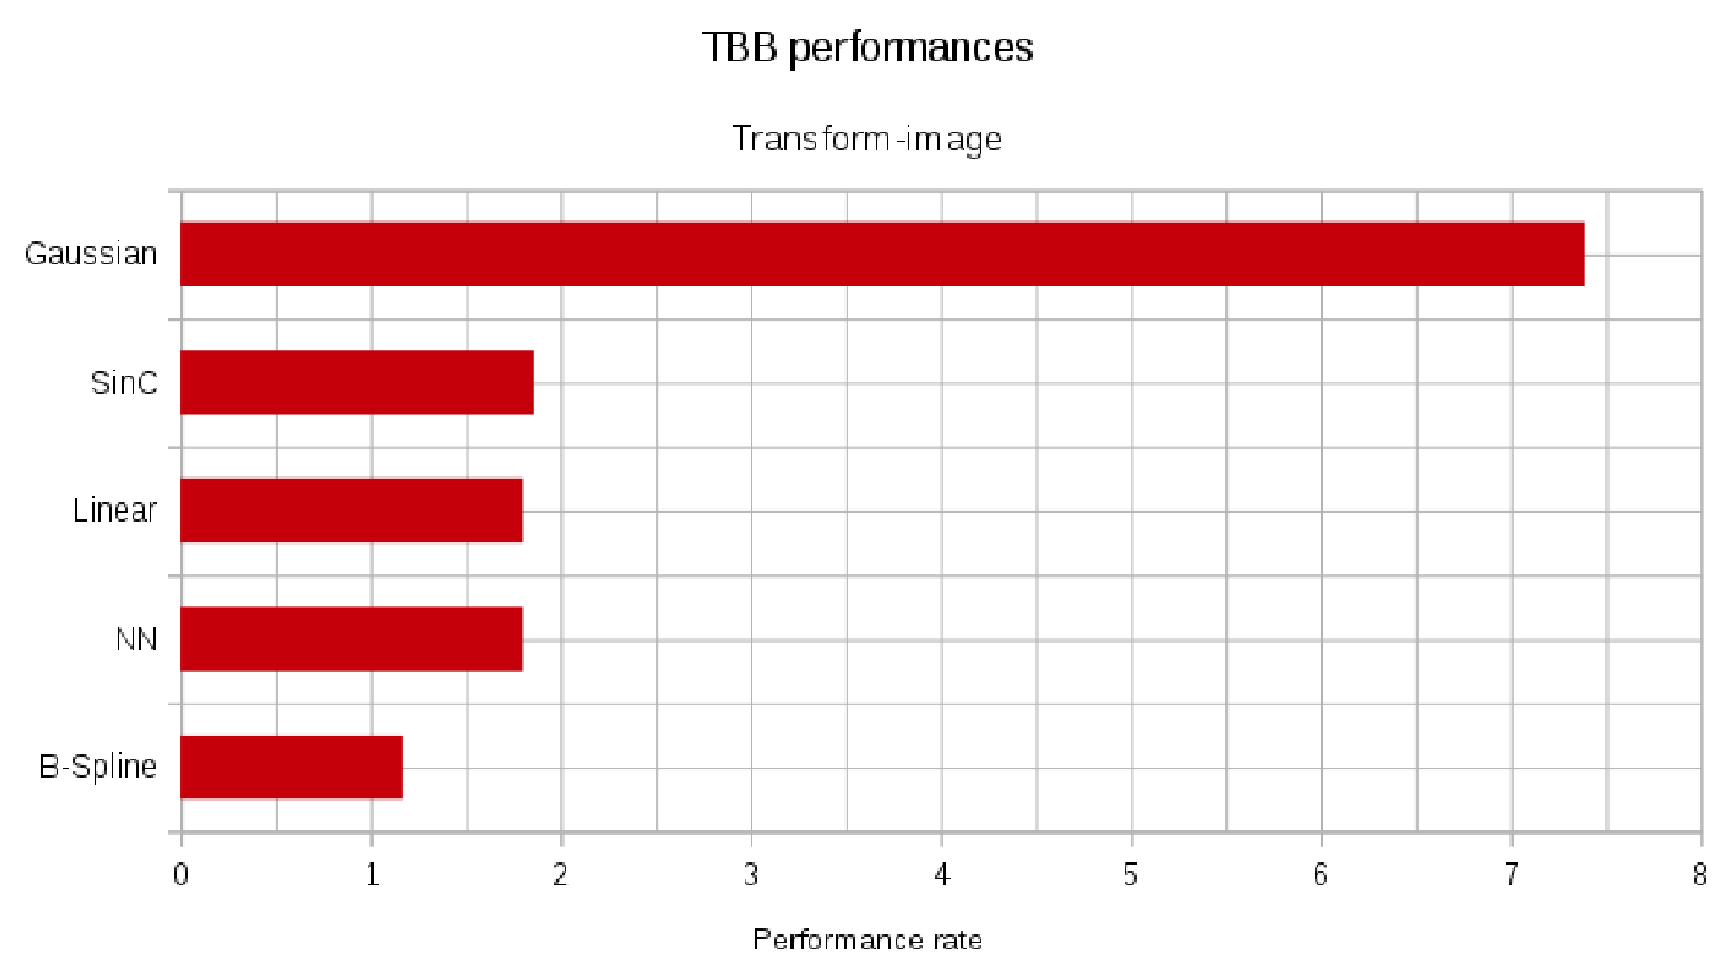
\includegraphics[width=9cm]{Reports/figures/performances_tbb_transform_image.eps}
			\end{center}	
			\caption{Améliorations apportées par TBB pour transform-image}
			\label{Améliorations apportées par TBB pour transform-image}
		\end{figure}~\par
		L'interpolation gaussienne est donc parfaitement parallélisée, ce qui n'est pas le cas des autres interpolations de \textit{transform-image}.
		
		\paragraph{Analyse des fuites de cache}
		Un deuxième critère intéressant à regarder, au travers du profilage, est la quantité de fuites de caches à l'exécution de la fonction étudiée. Bien que la parallélisation ne soit pas toujours optimale, elle peut néanmoins être parfois délaissée au profit d'une gestion de fuites de caches plus poussée.
		
		\subparagraph{Qu'est-ce qu'une fuite de cache?}
		\textit{?????}\\
		Ci-dessous est détaillé l'histogramme de la quantité des fuites de caches pour \textit{transform-image}, dans chaque mode d'interpolation:
			\begin{figure}[h!]
				\begin{center}
					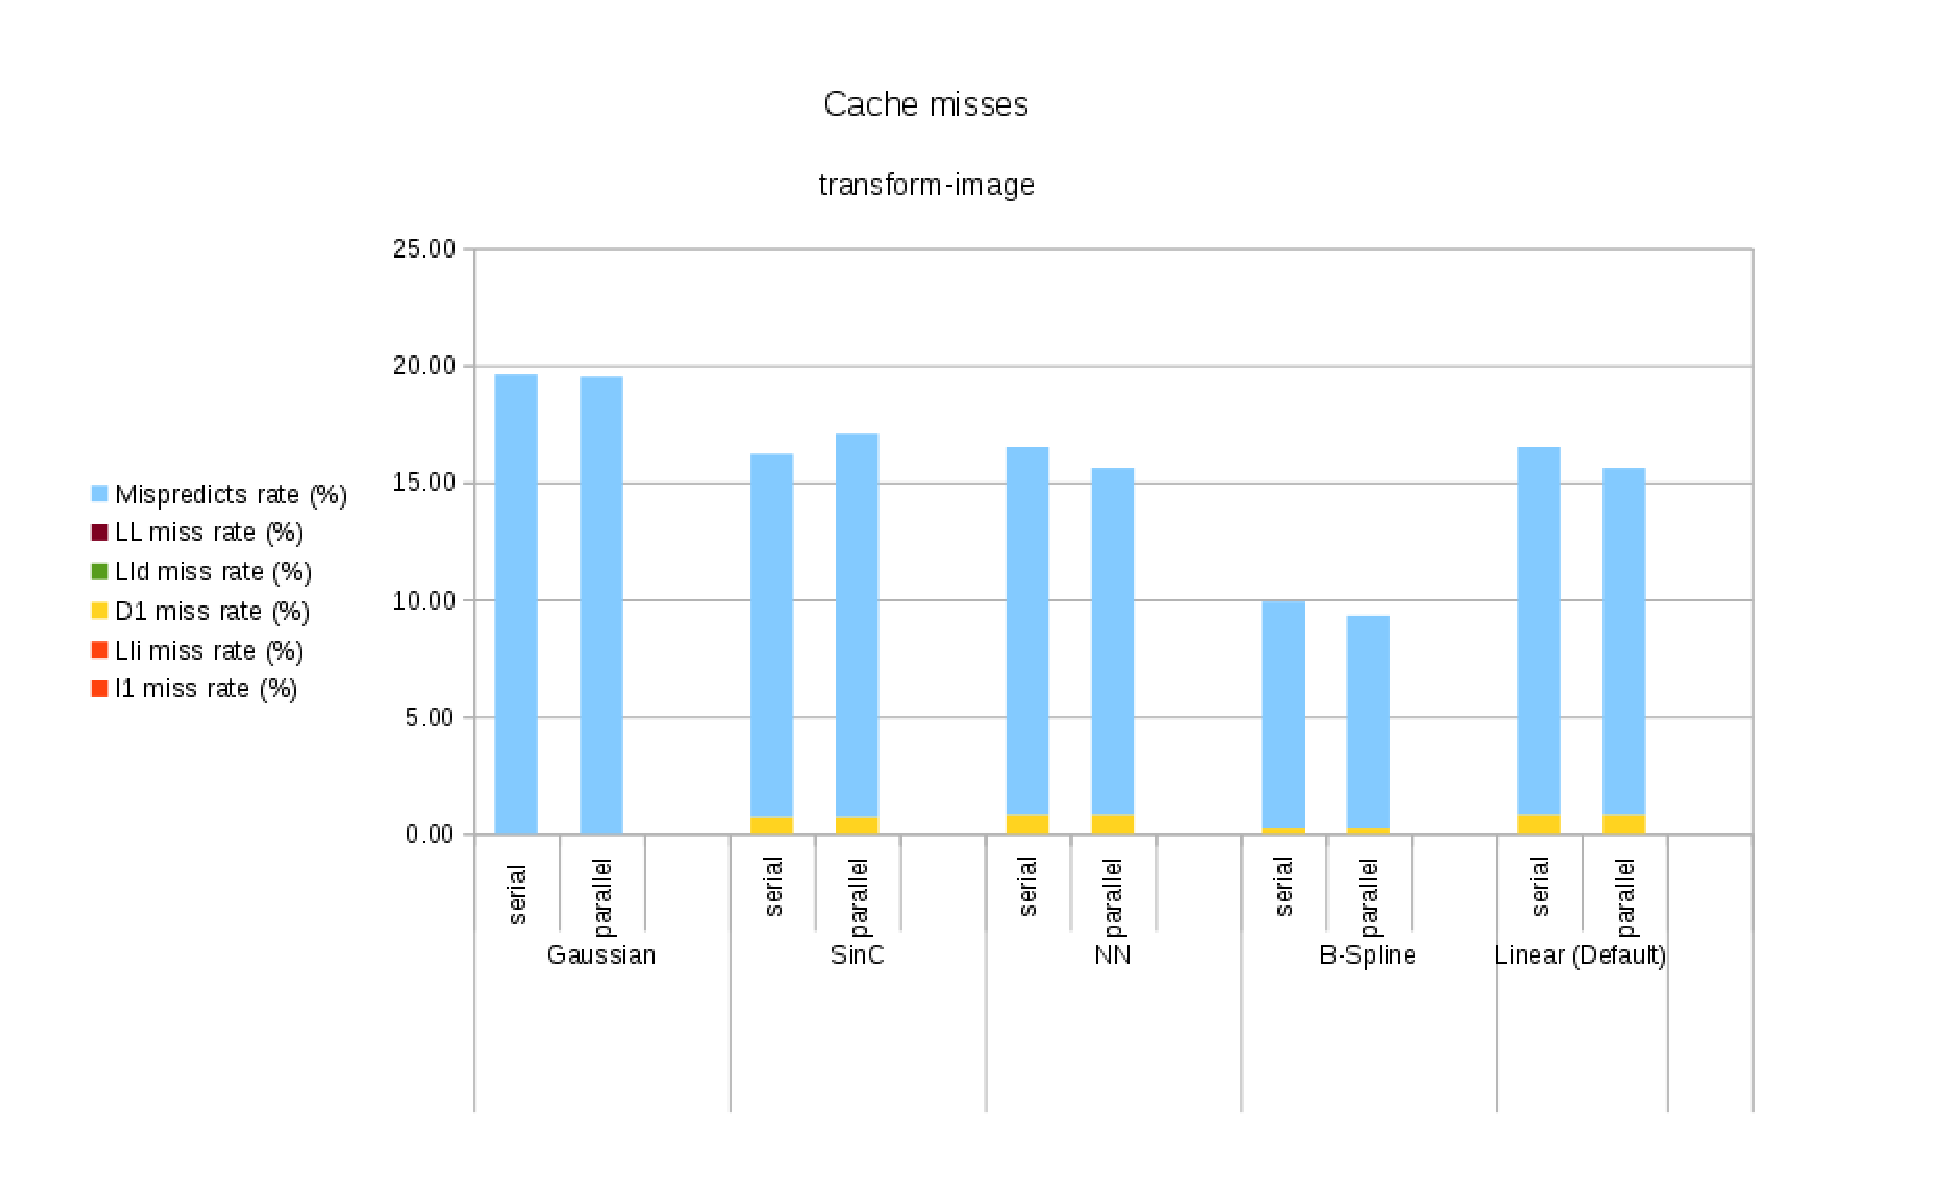
\includegraphics[width=15cm]{Reports/figures/cache_misses_transform_image.eps}
				\end{center}	
				\caption{Fuites de cache pour la fonction transform-image}
				\label{Fuites de cache pour la fonction transform-image}
			\end{figure}~\par
		Les valeurs données ci-dessus (en pourcentage) sont assez mal réparties, mais le faible "cache miss rate" (taux de fuites de caches) est très faible. Le seul taux non négligeable est celui des mauvaises prédictions de branche, qui peut être considéré comme une fuite de cache, mais un taux inférieur à 20 \% reste négligeable. 
		~\par
		MIRTK est donc bien conçu au niveau de la gestion de la mémoire cache, alors que le système de parallélisation est largement améliorable.

%	\subsection{Switch automatique de back-end}
%	Commandes prépocesseur pour indiquer au logiciel quel est le back-end à utiliser (ArrayFire ou Eigen) en fonction de l'opération souhaitée.

	\subsection{Benchmarking}
	(partie dépendante du déroulement du projet)\newline
	- Analyse des performances obtenues \newline
	- Comparaison avec le profilage initial ? \newline
	- Points où il y a eu des concessions (exemple: alourdir le code pour parvenir à un résultat précis)
	
\chapter{Améliorations et perspectives}
	\section{Au niveau technique...}
	\section{...mais pas seulement!}

\chapter*{Conclusion} % dans cet ordre
\addcontentsline{toc}{chapter}{Conclusion}
\chapter*{Sources}
\addcontentsline{toc}{chapter}{Sources}
\noindent
\url{https://biomedia.doc.ic.ac.uk/}  : image page de garde, partie du texte 1.1.2 \\
\url{http://www.imperial.ac.uk} : partie du texte 1.1.1 (Department of computing) et schéma stratégie du département\\
\url{https://fr.wikipedia.org/wiki/Imperial_College_London} : partie du texte 1.1.1 (Imperial College London)\\
\url{http://ric.uthscsa.edu/mango/papaya/index.html} : outil de visualisation d'images en format NIFTI
\renewcommand{\listfigurename}{Table des illustations}
\listoffigures
\addcontentsline{toc}{chapter}{Table des illustrations}
\chapter*{Glossaire}
\addcontentsline{toc}{chapter}{Glossaire}
\noindent
\textbf{Back-end:}\\ 
\textbf{Front-end:}\\
\textbf{MIRTK:}\\
\textbf{Profilage:} Différence avec le benchmarking ?\\
\textbf{Run-time:}\\
\textbf{Fuite de cache:}\\
\textbf{Benchmarking:} Différence avec le profiling ?\\
\textbf{Thread:}\\
\textbf{Prédiction de branche:}\\
\textbf{Fuite de cache:}\\


\chapter*{Annexes}
\addcontentsline{toc}{chapter}{Annexes}
\end{document}
